\documentclass[border=10pt]{standalone}
\usepackage{tikz}
\usetikzlibrary{arrows.meta,shapes,calc}

\begin{document}
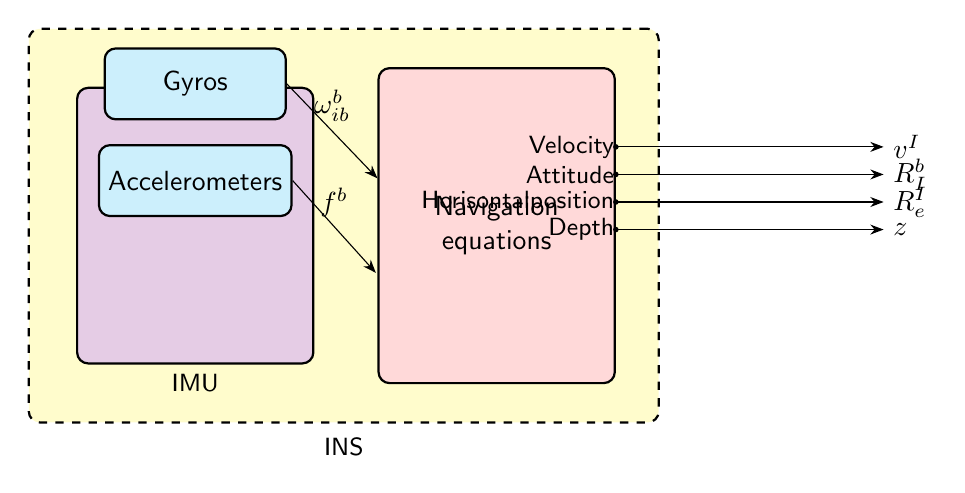
\begin{tikzpicture}[
    >=Stealth,
    font=\sffamily,
    block/.style={draw, rounded corners, thick, align=center},
    sensblock/.style={block, fill=cyan!20, minimum width=2.3cm, minimum height=0.9cm},
    labelstyle/.style={font=\sffamily\small},
    mathlabel/.style={font=\normalsize}
]

% Main INS container
\node[block, dashed, fill=yellow!20,
      minimum width=8cm, minimum height=5cm, anchor=center] (ins) at (0,0) {};

% IMU outer block inside INS
\node[block, fill=violet!20, minimum width=3cm, minimum height=3.5cm,
      anchor=west] (imu) at ([xshift=-3.4cm]ins.center) {};

\node[labelstyle, anchor=north] at (imu.south) {IMU};

% Gyros block
\node[sensblock, anchor=north] (gyros) at ([yshift=0.5cm]imu.north) {Gyros};

% Accelerometers block
\node[sensblock, anchor=north] (accel) at ([yshift=-0.3cm]gyros.south) {Acceler\-ometers};

% Navigation equations block
\node[block, fill=red!15, minimum width=3cm, minimum height=4cm,
      anchor=west] (nav) at ([xshift=0.8cm]imu.east) {Navigation\\equations};

% Label INS at bottom center of container
\node[labelstyle] at ([yshift=-0.3cm]ins.south) {INS};

% Arrows from IMU to Navigation block
\draw[->] (gyros.east) -- node[above, mathlabel] {$\omega_{ib}^b$}
      ($(nav.west)+(0,0.6)$);

\draw[->] (accel.east) -- node[above, mathlabel] {$f^{b}$}
      ($(nav.west)+(-0.02,-0.6)$);

% Right side output arrows from Navigation equations
% Define y positions relative to nav center
\coordinate (navright) at (nav.east);

% Vertical offsets for the four outputs
\def\yo{1.0}
\def\yd{0.35}

% Velocity
\coordinate (p1) at ($(navright)+(0,\yo)$);
\fill (p1) circle (1pt);
\draw[->] (p1) -- ++(3.4,0) node[mathlabel, anchor=west] {$v^{I}$};
\node[labelstyle, anchor=east] at ($(p1)+(0.1,0)$) {Velocity};

% Attitude
\coordinate (p2) at ($(navright)+(0,\yo-\yd)$);
\fill (p2) circle (1pt);
\draw[->] (p2) -- ++(3.4,0) node[mathlabel, anchor=west] {$R^{b}_{I}$};
\node[labelstyle, anchor=east] at ($(p2)+(0.1,0)$) {Attitude};

% Horizontal position
\coordinate (p3) at ($(navright)+(0,\yo-2*\yd)$);
\fill (p3) circle (1pt);
\draw[->] (p3) -- ++(3.4,0) node[mathlabel, anchor=west] {$R^{I}_{e}$};
\node[labelstyle, anchor=east] at ($(p3)+(0.1,0)$) {Horisontal\\position};

% Depth
\coordinate (p4) at ($(navright)+(0,\yo-3*\yd)$);
\fill (p4) circle (1pt);
\draw[->] (p4) -- ++(3.4,0) node[mathlabel, anchor=west] {$z$};
\node[labelstyle, anchor=east] at ($(p4)+(0.1,0)$) {Depth};

\end{tikzpicture}
\end{document}